% =====================================================================
%  Diapositivas (VERSIÓN COMPLETA ~20 min) — Efecto Mpemba cuántico en HPC
%  Charla conjunta Juan (teal) / Sebastián (naranja). 16:9.
%  Compilar DESDE esta carpeta:
%    pdflatex diapositivas_qmpe_20min && bibtex diapositivas_qmpe_20min && pdflatex x2
% =====================================================================
\documentclass[aspectratio=169,10pt]{beamer}
\usepackage[utf8]{inputenc}
\usepackage[T1]{fontenc}
\usepackage[spanish,es-noshorthands]{babel}
\usepackage{amsmath,amssymb,bm}
\usepackage{graphicx,booktabs}
\usepackage{xcolor}
\usepackage{listings}
\graphicspath{{../}}

\usetheme{default}
\setbeamertemplate{navigation symbols}{}
\setbeamertemplate{footline}[frame number]
\setbeamertemplate{itemize items}[circle]

\definecolor{juan}{RGB}{15,115,140}
\definecolor{seb}{RGB}{205,95,25}
\definecolor{ink}{RGB}{33,37,48}
\definecolor{soft}{RGB}{120,125,135}
\setbeamercolor{frametitle}{fg=ink}
\setbeamercolor{title}{fg=ink}
\setbeamercolor{structure}{fg=ink}
\setbeamercolor{normal text}{fg=ink}
\setbeamerfont{frametitle}{series=\bfseries}

\newcommand{\J}{\hfill\colorbox{juan}{\color{white}\scriptsize\bfseries~Juan~}}
\newcommand{\Sb}{\hfill\colorbox{seb}{\color{white}\scriptsize\bfseries~Sebastián~}}
\newcommand{\cj}[1]{\textcolor{juan}{\textbf{#1}}}
\newcommand{\cs}[1]{\textcolor{seb}{\textbf{#1}}}
\newcommand{\rss}{\rho_{\mathrm{ss}}}
\newcommand{\Lop}{\mathcal{L}}
\newcommand{\ket}[1]{\lvert #1\rangle}
\newcommand{\bra}[1]{\langle #1\rvert}
\newcommand{\dyad}[2]{\lvert #1\rangle\langle #2\rvert}

\lstdefinestyle{core}{
  basicstyle=\ttfamily\scriptsize,
  keywordstyle=\color{blue!55!black}\bfseries,
  commentstyle=\color{green!40!black}\itshape,
  stringstyle=\color{red!55!black},
  emph={pragma,omp,parallel,for,schedule,MPI_Reduce,MPI_Allgatherv,MPI_Init,
        executor,map,ThreadPoolExecutor},
  emphstyle=\color{seb}\bfseries,
  showstringspaces=false, columns=fullflexible, breaklines=true,
  keepspaces=true, tabsize=2,
}
\lstset{style=core}

\newcommand{\divider}[3]{%
  \begingroup
  \setbeamercolor{background canvas}{bg=#1}
  \begin{frame}[plain]
    \vfill\begin{center}
      {\color{white}\Large\bfseries #3}\\[4pt]{\color{white!85}\small #2}
    \end{center}\vfill
  \end{frame}
  \endgroup}

\title{\bfseries El efecto Mpemba cuántico en HPC}
\subtitle{Modos lentos, evolución temporal, trayectorias y redes tensoriales}
\author{\cj{Juan} \quad\textbar\quad \cs{Sebastián}}
\institute{\small Sistemas Distribuidos / HPC --- 2026}
\date{}

\begin{document}

{\setbeamertemplate{footline}{}
\begin{frame}[plain]
  \titlepage
  \begin{center}\small\textcolor{soft}{Versión completa ($\approx$20 min) ---
  implementación serial y paralela (OpenMP · MPI · hilos · CUDA), validación y escalado}\end{center}
\end{frame}}

\begin{frame}{Hoja de ruta}
  \begin{columns}[T]
  \begin{column}{0.5\textwidth}
    \begin{enumerate}[1.]
      \item \cj{De lo clásico (macro) a lo cuántico}
      \item \cj{T1 — Modos lentos del Liouvilliano}
      \item \cs{Evolución temporal (a): RK4 directo}
      \item \cs{Evolución temporal (b): Krylov}
    \end{enumerate}
  \end{column}
  \begin{column}{0.5\textwidth}
    \begin{enumerate}[1.]\setcounter{enumi}{4}
      \item \cs{Muchos cuerpos: trayectorias (MPI) + GPU}
      \item \cj{Muchos cuerpos: redes tensoriales}
      \item \cj{Conclusiones generales}
      \item \cs{Relevancia en el efecto macro/meso}
    \end{enumerate}
  \end{column}
  \end{columns}
  \vfill
  \begin{center}\small\textcolor{soft}{%
    \colorbox{juan}{\color{white}~Juan~} modos lentos · redes tensoriales \quad
    \colorbox{seb}{\color{white}~Sebastián~} evolución temporal · trayectorias · GPU}
  \end{center}
\end{frame}

% ====================================================================
\divider{juan}{Juan}{1 · De lo clásico a lo cuántico}

\begin{frame}{El efecto Mpemba: una anomalía de relajación\J}
  \begin{columns}[T]
  \begin{column}{0.56\textwidth}\small
    \textbf{Clásico (macro).} A veces el agua \emph{más caliente} se congela
    \emph{antes} que la templada; se observa también en coloides, granulares e imanes
    \cite{MpembaOsborne1969,LuRaz2017,Kumar2022,Bechhoefer2021,Teza2026}.
    \medskip

    \textbf{La idea no es la temperatura} sino la \cs{geometría}: si medimos una
    \emph{distancia al equilibrio}, la curva que parte \textbf{más lejos} puede
    \textbf{cruzar} a la cercana y llegar antes.
    \medskip

    \textbf{Cuántico.} En sistemas abiertos markovianos reaparece como un cruce de
    curvas de distancia al estado estacionario \cite{Carollo2021,Nava2024} --- y se
    puede \emph{predecir} con álgebra lineal.
  \end{column}
  \begin{column}{0.44\textwidth}\centering
    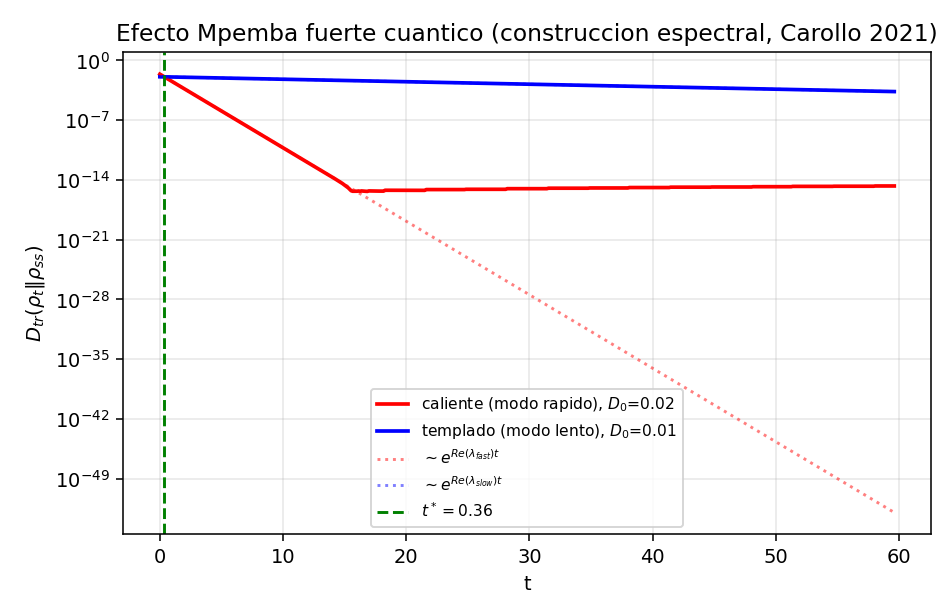
\includegraphics[width=\linewidth]{context/figures/03_mpemba_strong.png}\\
    {\scriptsize\textcolor{soft}{El cruce de curvas: el corazón del efecto.}}
  \end{column}
  \end{columns}
\end{frame}

\begin{frame}{La dinámica: ecuación maestra GKSL\J}
  \small
  Un sistema cuántico abierto markoviano evoluciona con la \textbf{ecuación de
  Lindblad (GKSL)} \cite{Lindblad1976,GKS1976,BreuerPetruccione2002}:
  \[
  \dot\rho=\Lop[\rho]=\underbrace{-i[H,\rho]}_{\text{coherente}}
   +\underbrace{\sum_\mu\Big(L_\mu\rho L_\mu^\dagger-\tfrac12\{L_\mu^\dagger L_\mu,\rho\}\Big)}_{\text{disipador (baño)}} .
  \]
  \begin{itemize}
    \item Modelo concreto: \textbf{cadena de Ising disipativa}
      $H=-J\sum Z_iZ_{i+1}-h\sum X_i$, con canales locales $\sigma^\pm$ (baño térmico).
    \item $\Lop$ es \textbf{lineal} en $\rho$ $\Rightarrow$ un \emph{superoperador} de
      dimensión $4^N\times4^N$. Ahí nace el reto de HPC: $4^N$ crece muy rápido.
    \item \cs{Clave:} los canales $\sigma^\pm$ locales \emph{no} llevan a Gibbs($H$);
      el estacionario $\rss$ es un estado de \emph{no-equilibrio} (núcleo de $\Lop$).
  \end{itemize}
\end{frame}

\begin{frame}{El espectro del Liouvilliano y el criterio de Mpemba\J}
  \small
  \textbf{Descomposición espectral} (autovalores $\lambda_k$, $\mathrm{Re}\,\lambda_k\le0$):
  \[
  \rho_t=\rss+\sum_{k\ge2}\, a_k\,e^{\lambda_k t}\,\hat r_k,\qquad
  a_k=\mathrm{Tr}(\hat l_k^\dagger\rho_0).
  \]
  \begin{itemize}
    \item La relajación es una \textbf{suma de modos} que decaen; a tiempos largos
      manda el \cs{modo lento} $\lambda_2$, escala $\tau=1/|\mathrm{Re}\,\lambda_2|$.
    \item \cs{Criterio de Mpemba (fuerte):} si $a_2=\mathrm{Tr}(\hat l_2^\dagger\rho_0)=0$,
      la preparación \emph{salta} el modo lento y relaja a la tasa rápida $\Rightarrow$
      adelanta a otra que sí lo tiene \cite{Carollo2021,Chattopadhyay2026}.
    \item La \textbf{no-normalidad} de $\Lop$ ($\Lop\Lop^\dagger\!\neq\!\Lop^\dagger\Lop$):
      los modos no son ortogonales $\Rightarrow$ permite el adelantamiento.
  \end{itemize}
\end{frame}

\begin{frame}{El espectro del Liouvilliano $\Lop$\J}
  \centering
  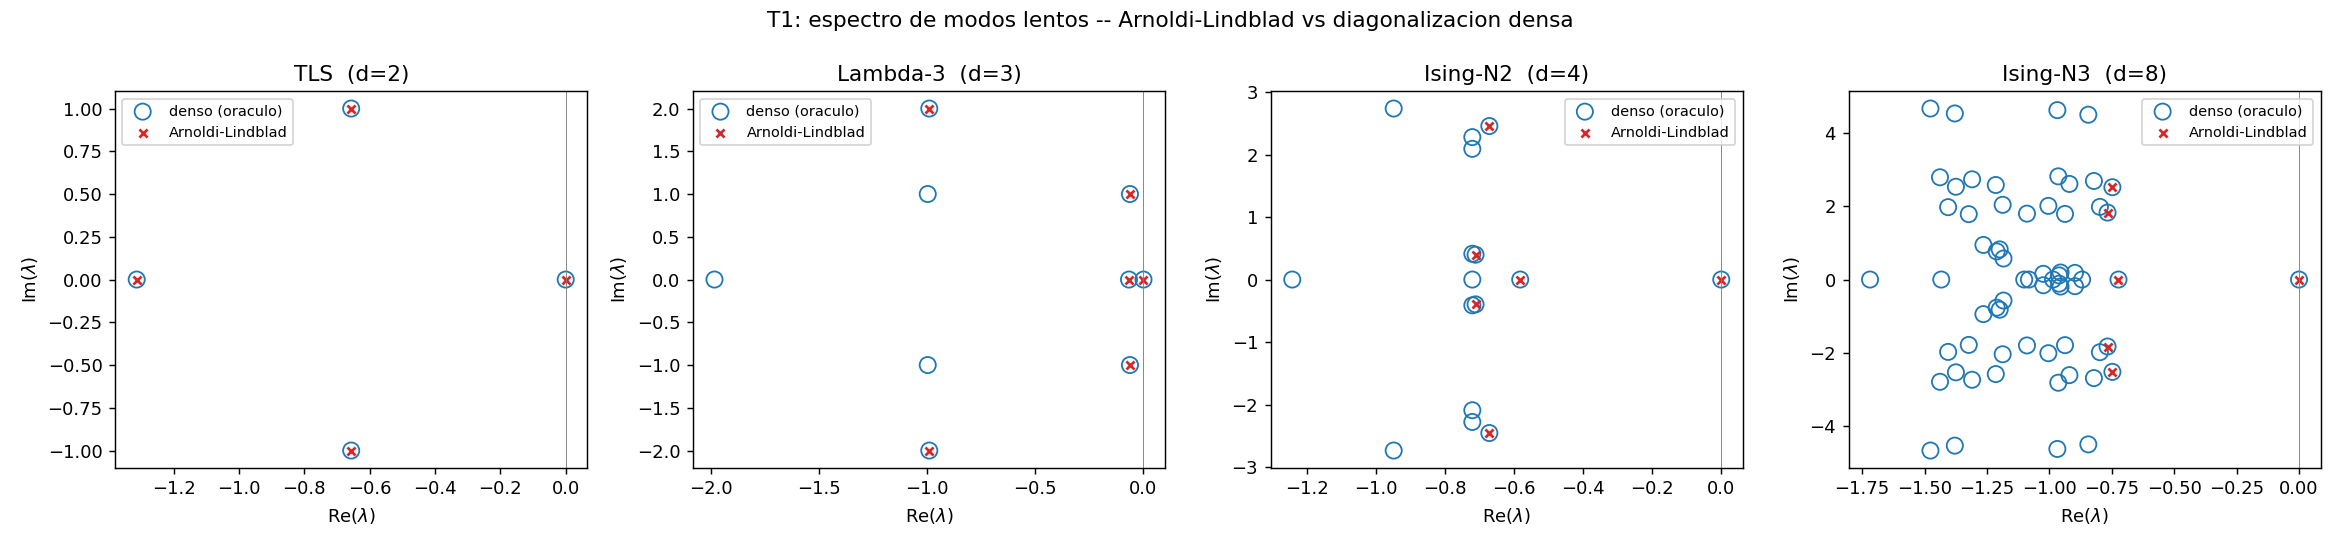
\includegraphics[height=0.68\textheight]{juan/T1/results/t1_eigs.png}\\[4pt]
  {\small Autovalores $\lambda_k$ en el plano complejo: $\lambda_1{=}0$ (estacionario
  $\rss$), todos con $\mathrm{Re}\,\lambda_k\le0$. El \cs{modo lento} $\lambda_2$ ---el
  más cercano a $0$--- fija la escala de relajación y controla el cruce de Mpemba.}
\end{frame}

\begin{frame}{Predicción del cruce: del espectro, \emph{sin evolucionar}\J}
  \small
  \textbf{Definimos dos preparaciones} (estados producto puros), ambas relajando al
  \emph{mismo} estacionario verdadero $\rss$:
  \begin{itemize}\small
    \item $\rho_A=\ket{+}^{\otimes N}$, con $\ket{+}=\tfrac{1}{\sqrt2}(\ket0+\ket1)$ \;---\; \cs{parte LEJOS}.
    \item $\rho_B=\ket{0}^{\otimes N}$ \;---\; \cs{parte CERCA}.
  \end{itemize}
  \smallskip
  Con el \textbf{espectro} (de T1: $\lambda_2,\hat l_2$) y los \textbf{solapamientos}
  $a_k=\mathrm{Tr}(\hat l_k^\dagger\rho_0)$ \,---\,\emph{solo una traza, sin integrar}---
  ya conocemos el destino de cada estado:
  \begin{center}\renewcommand{\arraystretch}{1.05}
  \begin{tabular}{lcc}
  \toprule
  estado & $D_0$ (arranque) & $|a_2|$ \;(peso del modo lento $\lambda_2{=}{-}0.70$) \\
  \midrule
  $\ket{+}^{\otimes N}$ (lejos) & \textbf{0.99} & \textbf{0.13} \\
  $\ket{0}^{\otimes N}$ (cerca) & 0.84 & 0.50 \\
  \bottomrule
  \end{tabular}\end{center}
  \smallskip
  \begin{center}\colorbox{seb!12}{\parbox{0.93\textwidth}{\centering\small
  $\ket{+}$ \textbf{arranca más alto} ($\times1.18$) pero \textbf{pesa menos en el modo
  lento} (asintótico $\times0.27$) $\;\Rightarrow\;$
  \cs{cruce garantizado}, con $t^*_{\rm pred}\!\approx\!0.68$, \emph{antes de resolver
  la dinámica}. Las tareas T2/T3 solo lo \emph{confirman}.}}\end{center}
\end{frame}

% ====================================================================
\divider{juan}{Juan}{2 · T1 — Modos lentos del Liouvilliano}

\begin{frame}{T1 — Framework y método numérico\J}
  \small
  \textbf{Objetivo.} Obtener $\lambda_2,\lambda_3,\dots$ y los solapamientos $a_k$
  \emph{sin diagonalizar} la matriz $4^N\times4^N$ (inviable en denso).
  \medskip

  \textbf{Método: Arnoldi sobre el propagador} $P(\tau)=e^{\tau\Lop}$
  \cite{Minganti2018,Lehoucq1998,Balay2023}.
  \begin{itemize}
    \item Los modos \emph{lentos} de $\Lop$ (interiores, cerca de 0) son los
      \emph{dominantes} de $P$ ($\mu_k=e^{\tau\lambda_k}$) $\Rightarrow$ Arnoldi los
      extrae \textbf{primero}: \emph{``faster than the clock''}.
    \item La acción de $P$ es \cs{matrix-free}: se integra $\dot V=\Lop[V]$ con RK4,
      sin formar $\Lop$.
  \end{itemize}
\end{frame}

\begin{frame}[fragile]{T1 — Núcleo: serial \textbar\ paralelo (MPI+OpenMP)\J}
  \begin{columns}[T]
  \begin{column}{0.46\textwidth}\centering\textbf{\small Serial}
\begin{lstlisting}[language=C++]
// producto C = A*B
for (int i=0;i<d;++i)
 for (int k=0;k<d;++k){
  cd a=A[i*d+k];
  for (int j=0;j<d;++j)
   C[i*d+j]+=a*B[k*d+j];
 }
\end{lstlisting}
  \end{column}
  \begin{column}{0.54\textwidth}\centering\textbf{\small Paralelo (datos)}
\begin{lstlisting}[language=C++]
#pragma omp parallel for        // intranodo
for (int i=rd.lo;i<rd.hi;++i)   // bloque del rango
 for (int k=0;k<d;++k){
  cd a=A[i*d+k];
  for (int j=0;j<d;++j)
   C[i*d+j]+=a*B[k*d+j];
 }
MPI_Allgatherv(...);            // reune C (internodo)
\end{lstlisting}
  \end{column}
  \end{columns}
  \vfill
  {\small \textbf{Dos niveles}: cada \cs{rango MPI} calcula un \emph{bloque de filas},
  \cs{OpenMP} lo reparte entre hilos, y \cs{MPI\_Allgatherv} reconstruye la matriz.
  El SpMV de Arnoldi llama a este núcleo.}
\end{frame}

\begin{frame}{T1 — Implementación, escalado y validación\J}
  \begin{columns}[T]
  \begin{column}{0.5\textwidth}\centering
    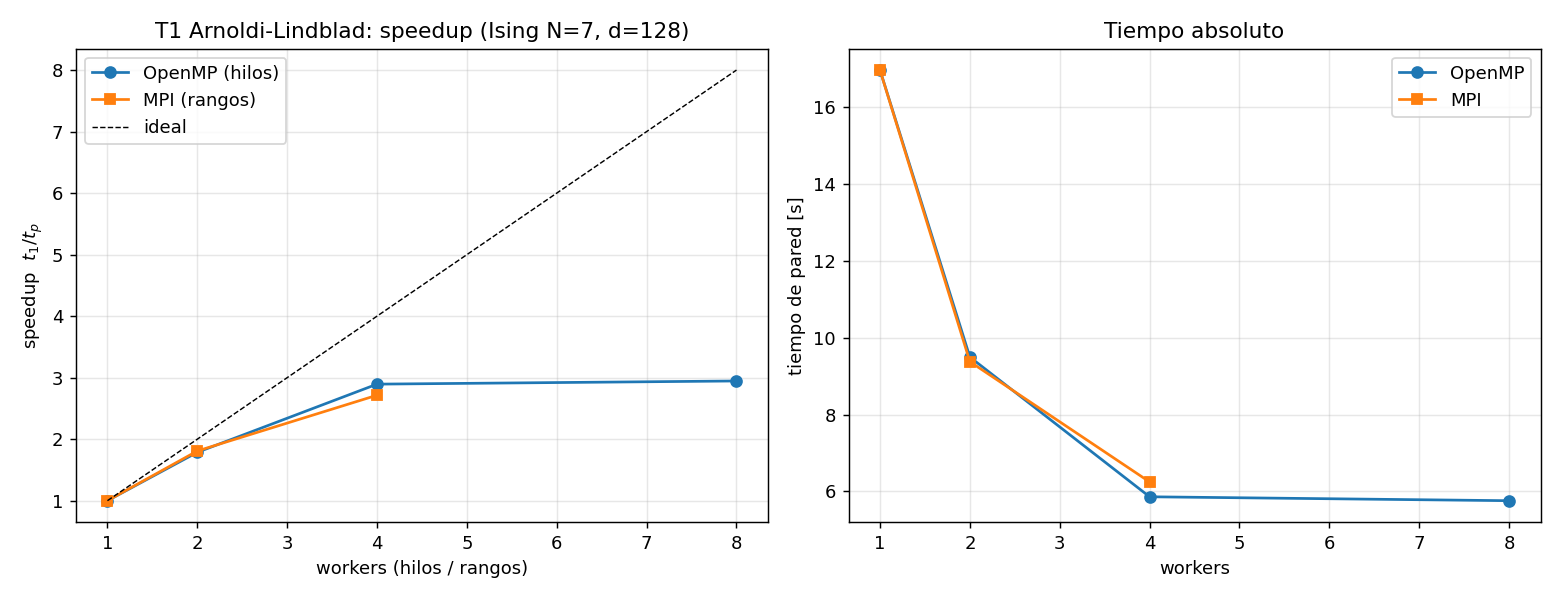
\includegraphics[width=\linewidth]{juan/T1/results/t1_scaling.png}\\
    {\scriptsize\textcolor{soft}{Escalado fuerte (Ising $N=7$, $d=128$).}}
  \end{column}
  \begin{column}{0.5\textwidth}\small
    \textbf{Computacional.}
    \begin{itemize}\small
      \item OpenMP $\,2.9\times\,$ / MPI $\,2.7\times\,$ (4 workers); \emph{plateau} en
        los núcleos físicos.
      \item SpMV \emph{memory-bound} y $\Lop$ \cs{acoplado} $\Rightarrow$ comunicación
        \texttt{Allgatherv}: es el caso \emph{menos} paralelizable.
    \end{itemize}
    \textbf{Validación / física.}
    \begin{itemize}\small
      \item Error en $\lambda$ lentos: $10^{-13}$–$10^{-5}$ vs denso.
      \item \emph{Faster-than-the-clock} hasta $8.8\times$ en SpMV.
      \item Da el $\lambda_2$ y el $a_2$ que \cs{determinan el cruce} de Mpemba.
    \end{itemize}
  \end{column}
  \end{columns}
\end{frame}

% ====================================================================
\divider{seb}{Sebastián}{3 · Evolución temporal (a): RK4 directo}

\begin{frame}{T2a — Framework y discretización\Sb}
  \small
  \textbf{Framework.} Integrar $\dot\rho=\Lop[\rho]$ desde una preparación $\rho_0$ y
  trazar la distancia $D_{HS}(\rho_t\|\rss)$ al estacionario.
  \medskip

  \textbf{Discretización: Runge--Kutta 4 (RK4).} Con paso $\Delta t$,
  \[
  \rho_{n+1}=\rho_n+\tfrac{\Delta t}{6}(k_1{+}2k_2{+}2k_3{+}k_4),\quad k_i=\Lop[\,\cdot\,],
  \]
  y la acción \cs{matrix-free}
  $\Lop[V]=-i(HV{-}VH)+\sum_\mu(L_\mu V L_\mu^\dagger-\tfrac12\{L_\mu^\dagger L_\mu,V\})$.
  \begin{itemize}\small
    \item Orden global $\mathcal{O}(\Delta t^4)$; coste por paso $\mathcal{O}(N d^3)$
      (domina el \cs{producto de matrices} densas).
  \end{itemize}
\end{frame}

\begin{frame}{T2a — Justificación de la paralelización (OpenMP)\Sb}
  \small
  \begin{itemize}
    \item \textbf{Patrón:} miles de pasos con \textbf{dependencia temporal estricta}
      ($\rho_{n+1}$ necesita $\rho_n$) $\Rightarrow$ \emph{no} se paraleliza entre pasos.
    \item El paralelismo disponible está \emph{dentro} del paso, en el \texttt{matmul}:
      datos regulares de tamaño moderado que caben en un nodo.
    \item $\Rightarrow$ paradigma natural \cs{OpenMP} (memoria compartida, sin halo).
      \textbf{MPI} sería contraproducente (comunicación en cada uno de los miles de
      pasos); \textbf{CUDA} ayuda pero requiere GPU (lo vemos en la sección 5).
    \item \textbf{Correctitud:} serial y paralelo dan el \emph{mismo} estado final a
      precisión de máquina (el observable $D_{HS}$ coincide).
  \end{itemize}
\end{frame}

\begin{frame}[fragile]{T2a — Núcleo: serial \textbar\ paralelo (OpenMP)\Sb}
  \begin{columns}[T]
  \begin{column}{0.48\textwidth}\centering\textbf{\small Serial}
\begin{lstlisting}[language=C++]
Mat matmul(A,B,d){
 Mat C(d*d);
 for(int i=0;i<d;++i)
  for(int k=0;k<d;++k){
   cd a=A[i*d+k];
   for(int j=0;j<d;++j)
    C[i*d+j]+=a*B[k*d+j];}
 return C;}
\end{lstlisting}
  \end{column}
  \begin{column}{0.52\textwidth}\centering\textbf{\small Paralelo}
\begin{lstlisting}[language=C++]
Mat matmul(A,B,d){
 Mat C(d*d);
 #pragma omp parallel for schedule(static)
 for(int i=0;i<d;++i)
  for(int k=0;k<d;++k){
   cd a=A[i*d+k];
   for(int j=0;j<d;++j)
    C[i*d+j]+=a*B[k*d+j];}
 return C;}
\end{lstlisting}
  \end{column}
  \end{columns}
  \vfill
  {\small Una \cs{\#pragma omp parallel for} reparte las filas $i$ entre hilos. El
  \emph{mismo} binario, con distinto \texttt{OMP\_NUM\_THREADS}, da serie vs paralelo.}
\end{frame}

\begin{frame}{T2a — Escalado y validación numérica\Sb}
  \begin{columns}[T]
  \begin{column}{0.5\textwidth}\centering
    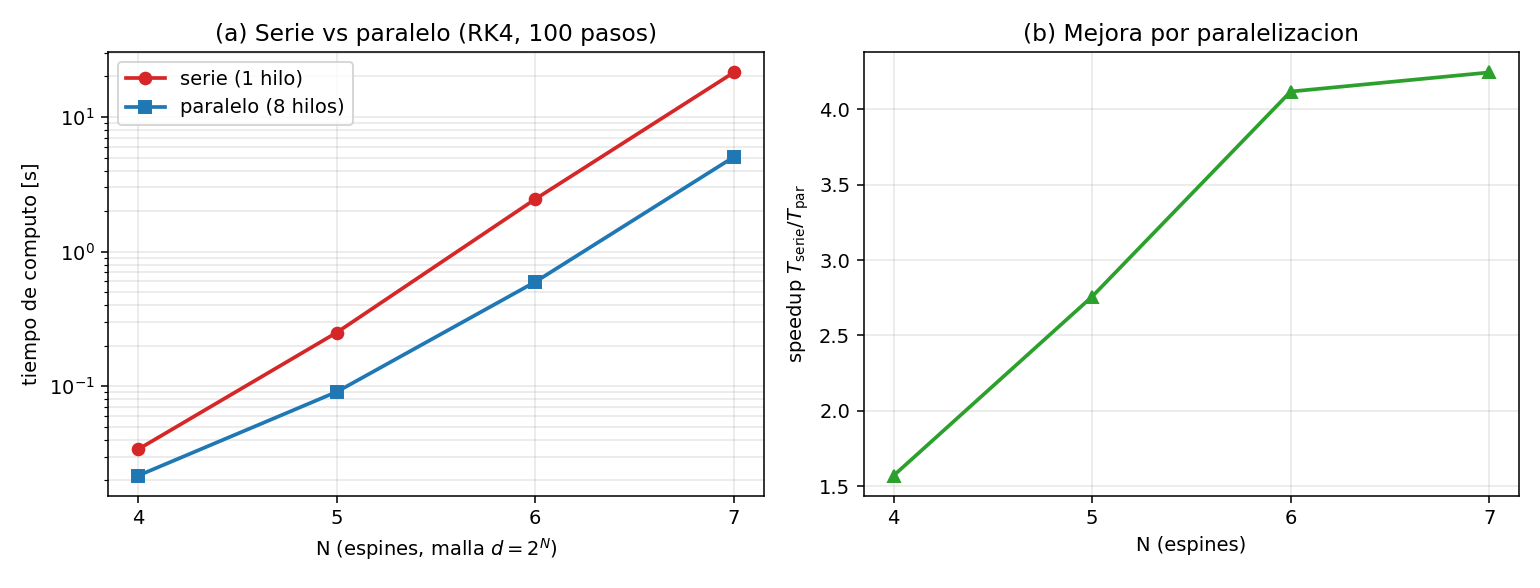
\includegraphics[width=\linewidth]{T2/a_integracion_directa/results/fig_t2a_serial_parallel.png}\\
    {\scriptsize\textcolor{soft}{Serie vs paralelo vs $N$: speedup $\to\!4\times$ (sublineal).}}
  \end{column}
  \begin{column}{0.5\textwidth}\centering
    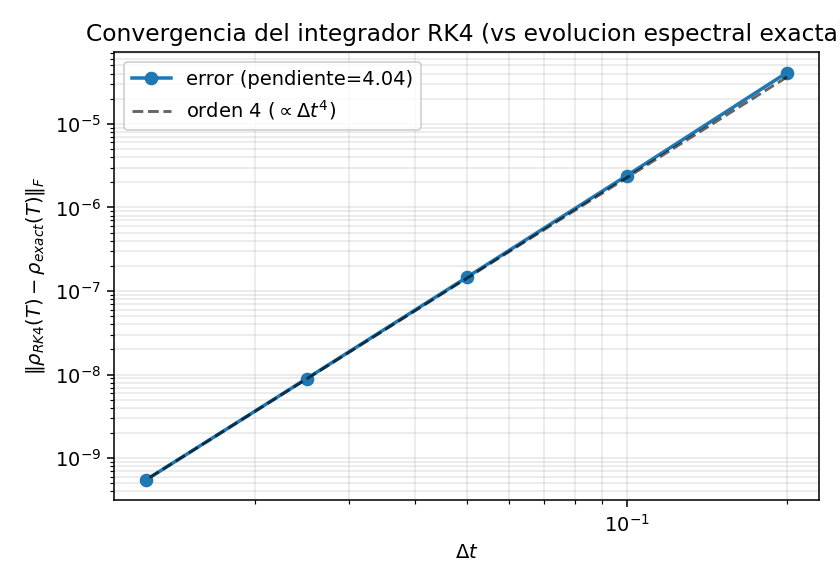
\includegraphics[width=\linewidth]{T2/a_integracion_directa/results/fig_t2a_convergence.png}\\
    {\scriptsize\textcolor{soft}{Convergencia orden 4 ($\approx4.04$) vs solución exacta.}}
  \end{column}
  \end{columns}
  \vfill
  {\small Speedup OpenMP \emph{bandwidth-bound}; el integrador queda validado a orden 4
  contra la evolución espectral exacta.}
\end{frame}

\begin{frame}{T2a — Resultado físico: el cruce de Mpemba\Sb}
  \begin{columns}[T]
  \begin{column}{0.55\textwidth}\centering
    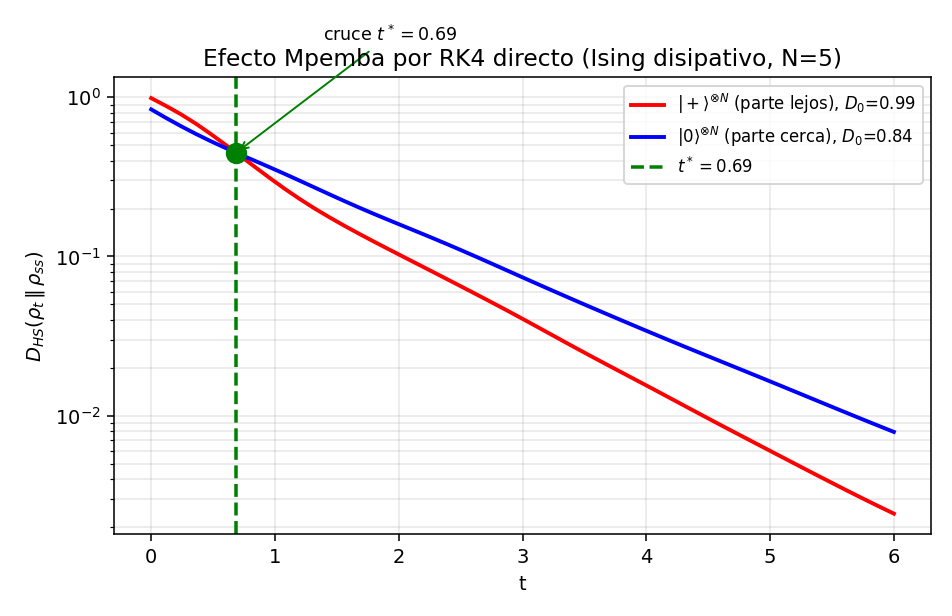
\includegraphics[width=0.92\linewidth]{T2/a_integracion_directa/results/fig_t2a_mpemba.png}
  \end{column}
  \begin{column}{0.45\textwidth}\small
    Dos preparaciones del mismo modelo: $\ket{+}^{\otimes N}$ (parte lejos) y
    $\ket{0}^{\otimes N}$ (parte cerca), distancia al \cs{estacionario verdadero} $\rss$.
    \medskip

    La que parte lejos (roja) \textbf{adelanta} a la cercana (azul) en
    \cs{$t^*\approx0.69$}: ahí está el efecto Mpemba, reproducido por RK4.
  \end{column}
  \end{columns}
\end{frame}

% ====================================================================
\divider{seb}{Sebastián}{4 · Evolución temporal (b): Krylov}

\begin{frame}{T2b — Método: acción del exponencial\Sb}
  \small
  \textbf{Idea.} En vez de integrar paso a paso, aplicar la \cs{acción del exponencial}
  $\rho(t{+}\tau)=e^{\tau\Lop}[\rho]$ (solución \emph{exacta} en un paso $\tau$).
  \begin{itemize}
    \item $e^{\tau\Lop}$ es enorme $\Rightarrow$ se proyecta en un subespacio de
      \textbf{Krylov} $\mathcal{K}_m$ (Arnoldi, $m\sim30$) y se exponencia la matriz
      pequeña $m\times m$ \cite{Sidje1998,AlMohyHigham2011}.
    \item \emph{Mismo hotspot} que RK4 (el \texttt{matmul} de $\Lop[\cdot]$)
      $\Rightarrow$ \textbf{misma paralelización OpenMP} y escalado equivalente.
    \item Ventajas: pasos $\tau$ grandes, \textbf{incondicionalmente estable}, ideal
      para llegar al estacionario.
  \end{itemize}
\end{frame}

\begin{frame}{T2b — El resultado central: precisión por unidad de trabajo\Sb}
  \begin{columns}[T]
  \begin{column}{0.55\textwidth}\centering
    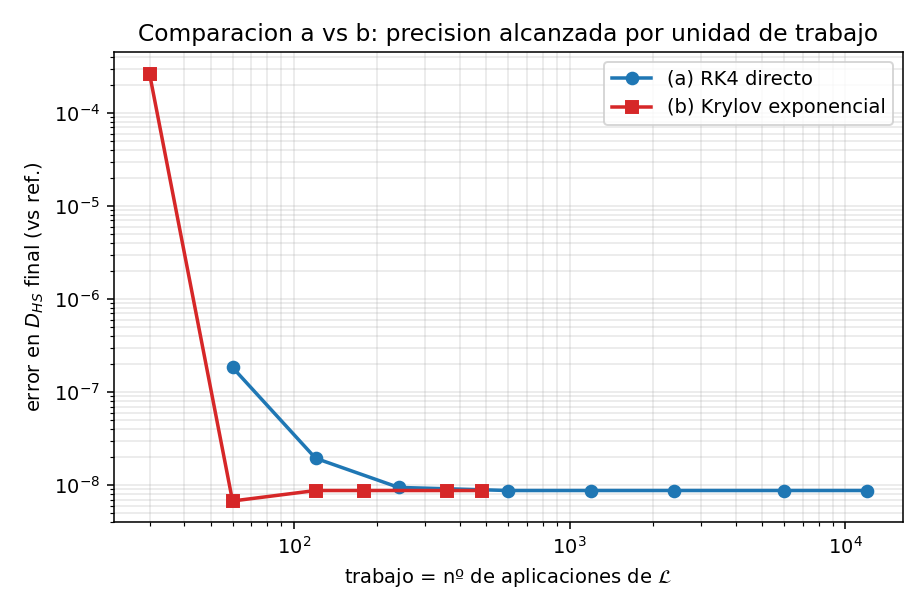
\includegraphics[width=0.96\linewidth]{T2/b_accion_exponencial/results/fig_t2b_method_compare.png}
  \end{column}
  \begin{column}{0.45\textwidth}\small
    A igual \textbf{trabajo} (nº de aplicaciones de $\Lop$, independiente de la
    máquina), \cs{Krylov es $\sim25\times$ más preciso} que RK4.
    \medskip

    Convergencia \emph{super-algebraica} en $m$ frente a la algebraica
    ($\propto\Delta t^4$) de RK4. RK4 sigue siendo mejor para trayectorias densas o
    $\Lop$ dependiente del tiempo.
  \end{column}
  \end{columns}
\end{frame}

\begin{frame}{T2b — El cruce de Mpemba por Krylov\Sb}
  \begin{columns}[T]
  \begin{column}{0.55\textwidth}\centering
    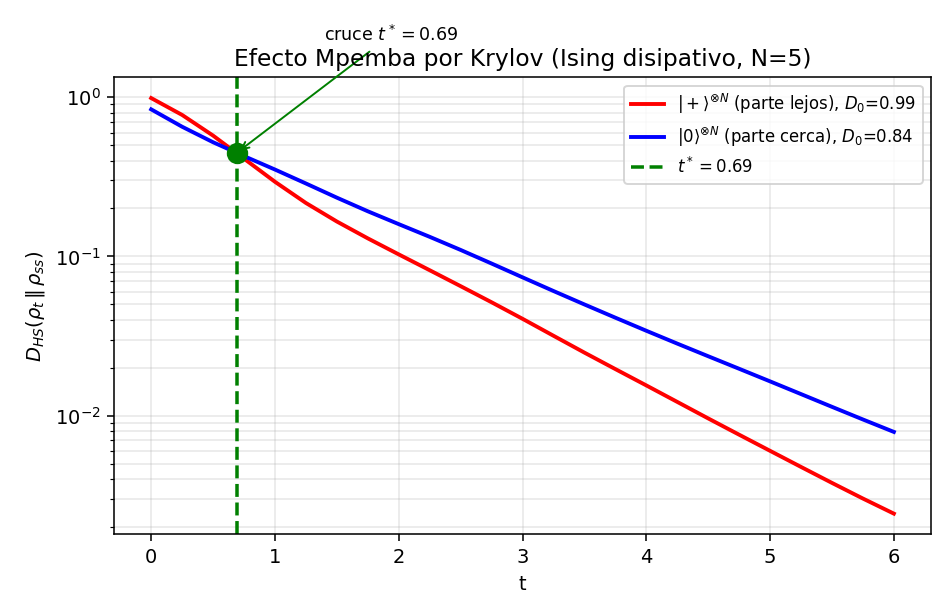
\includegraphics[width=0.9\linewidth]{T2/b_accion_exponencial/results/fig_t2b_mpemba.png}
  \end{column}
  \begin{column}{0.45\textwidth}\small
    \cs{Mismo cruce, $t^*\approx0.69$}, idéntico a RK4 (acuerdo a $10^{-10}$ en
    $D_{HS}$ final).
    \medskip

    Mensaje: el cruce es \textbf{física}, no un artefacto del integrador; y Krylov lo
    obtiene con pasos de tiempo grandes.
  \end{column}
  \end{columns}
\end{frame}

% ====================================================================
\divider{seb}{Sebastián}{5 · Muchos cuerpos: trayectorias (MPI) + GPU}

\begin{frame}[fragile]{T3 — Trayectorias: método y núcleo serial \textbar\ paralelo\Sb}
  \small
  \textbf{Monte Carlo wavefunction} \cite{Daley2014,Johansson2013}: propagar $M$ estados
  \emph{puros} $\ket\psi\in\mathbb{C}^d$ (memoria $d$, no $d^2$) con $H_{\rm eff}$ y
  \emph{saltos}, y promediar $\rho=\mathbb{E}[\dyad{\psi}{\psi}]$. \cs{Embarrassingly parallel}.
  \begin{columns}[T]
  \begin{column}{0.46\textwidth}\centering\textbf{\scriptsize Serial}
\begin{lstlisting}[language=C++]
for(int tr=0;tr<M;++tr){
 psi=ket0;
 for(paso) RK4_Heff+salto(psi);
 acc += |psi><psi|;
}
rho = acc / M;
\end{lstlisting}
  \end{column}
  \begin{column}{0.54\textwidth}\centering\textbf{\scriptsize Paralelo (MPI)}
\begin{lstlisting}[language=C++]
int my_M = M/size + ...;     // reparto
for(int tr=0;tr<my_M;++tr){
 ... acc_local += |psi><psi|;
}
MPI_Reduce(acc_local,acc,MPI_SUM,0);
if(rank==0) rho = acc / M;   // 1 sola colectiva
\end{lstlisting}
  \end{column}
  \end{columns}
  \vfill
  {\small Cada rango integra su lote \emph{sin comunicación}; una única \cs{MPI\_Reduce}
  promedia. Sin halo ni dependencias $\Rightarrow$ escalado casi ideal y multinodo.}
\end{frame}

\begin{frame}{T3 — Escalado y convergencia estadística\Sb}
  \begin{columns}[T]
  \begin{column}{0.5\textwidth}\centering
    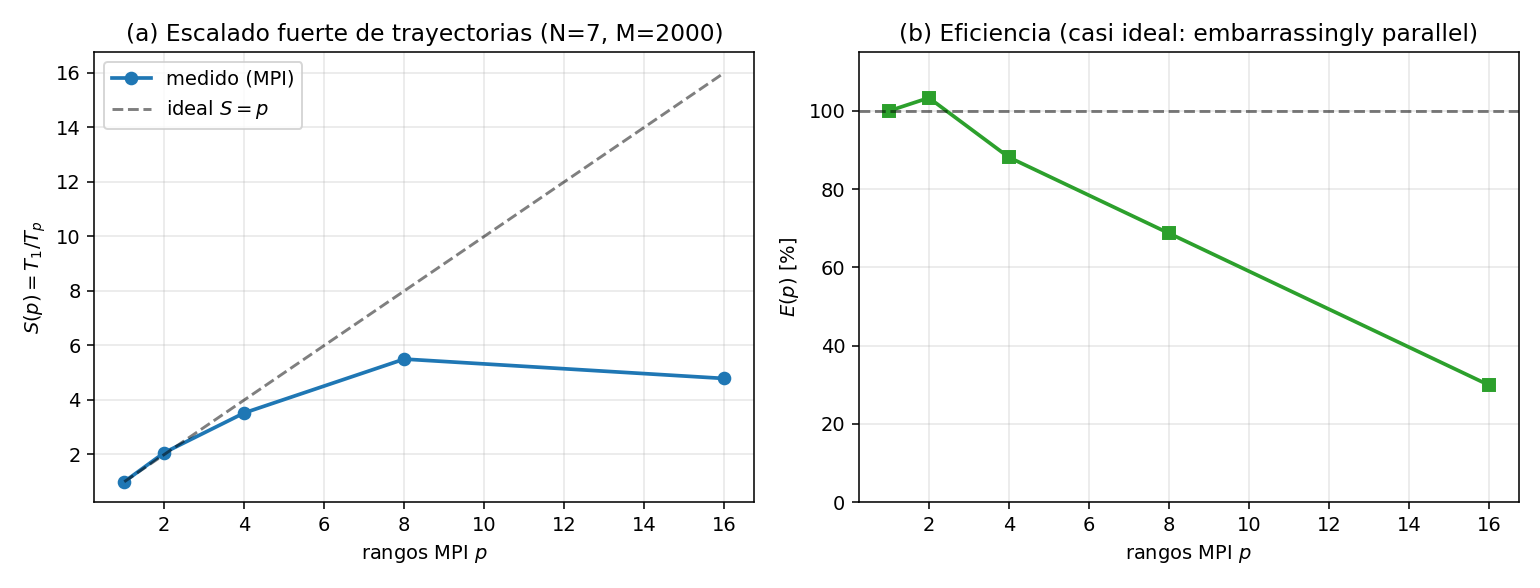
\includegraphics[width=\linewidth]{T3/integration/results/fig_t3_speedup.png}\\
    {\scriptsize\textcolor{soft}{Escalado fuerte MPI: \emph{casi ideal} ($S\approx5.5$).}}
  \end{column}
  \begin{column}{0.5\textwidth}\centering
    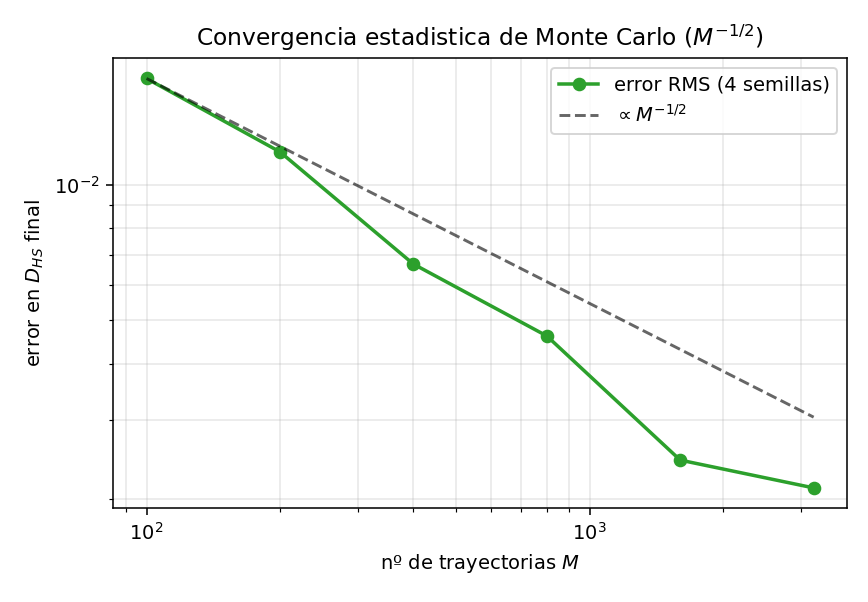
\includegraphics[width=\linewidth]{T3/integration/results/fig_t3_error_M.png}\\
    {\scriptsize\textcolor{soft}{Convergencia estadística $\propto M^{-1/2}$.}}
  \end{column}
  \end{columns}
  \vfill
  {\small Contraste con el OpenMP sublineal de T2: \cs{el patrón de cómputo dicta el
  paradigma}. Precisión: una cifra más $\Rightarrow$ $100\times$ trayectorias (pero hay
  paralelismo de sobra).}
\end{frame}

\begin{frame}{T3 — Resultado físico: el cruce de Mpemba\Sb}
  \begin{columns}[T]
  \begin{column}{0.55\textwidth}\centering
    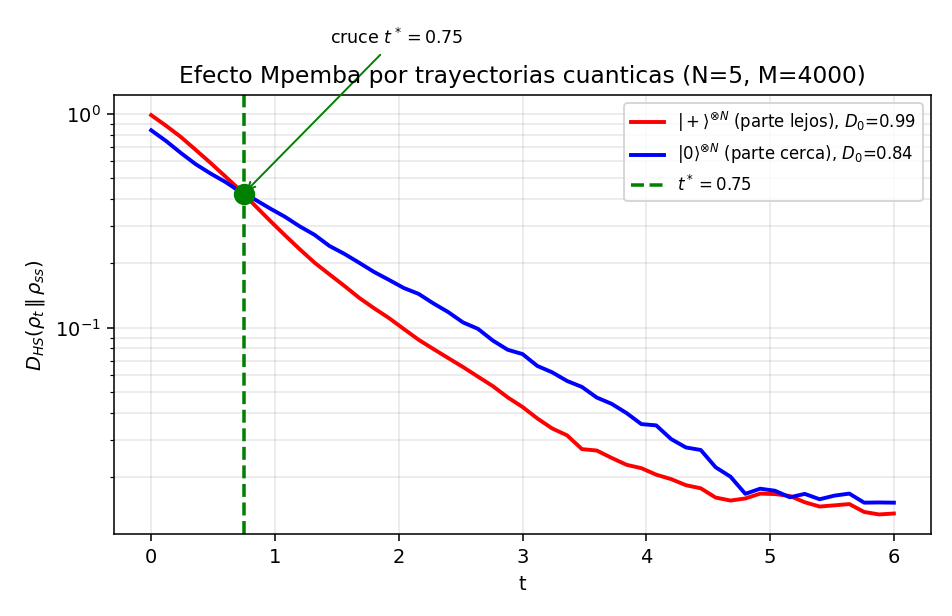
\includegraphics[width=0.92\linewidth]{T3/integration/results/fig_t3_mpemba.png}
  \end{column}
  \begin{column}{0.45\textwidth}\small
    También el método \emph{estocástico} captura el cruce: la curva que parte lejos
    \textbf{adelanta} a la cercana en \cs{$t^*\approx0.75$}.
    \medskip

    El ruido del suelo a tiempos largos es el error estadístico $M^{-1/2}$ del Monte
    Carlo.
  \end{column}
  \end{columns}
\end{frame}

\begin{frame}{T3 — Aceleración en GPU (CUDA / T4)\Sb}
  \begin{columns}[T]
  \begin{column}{0.5\textwidth}\centering
    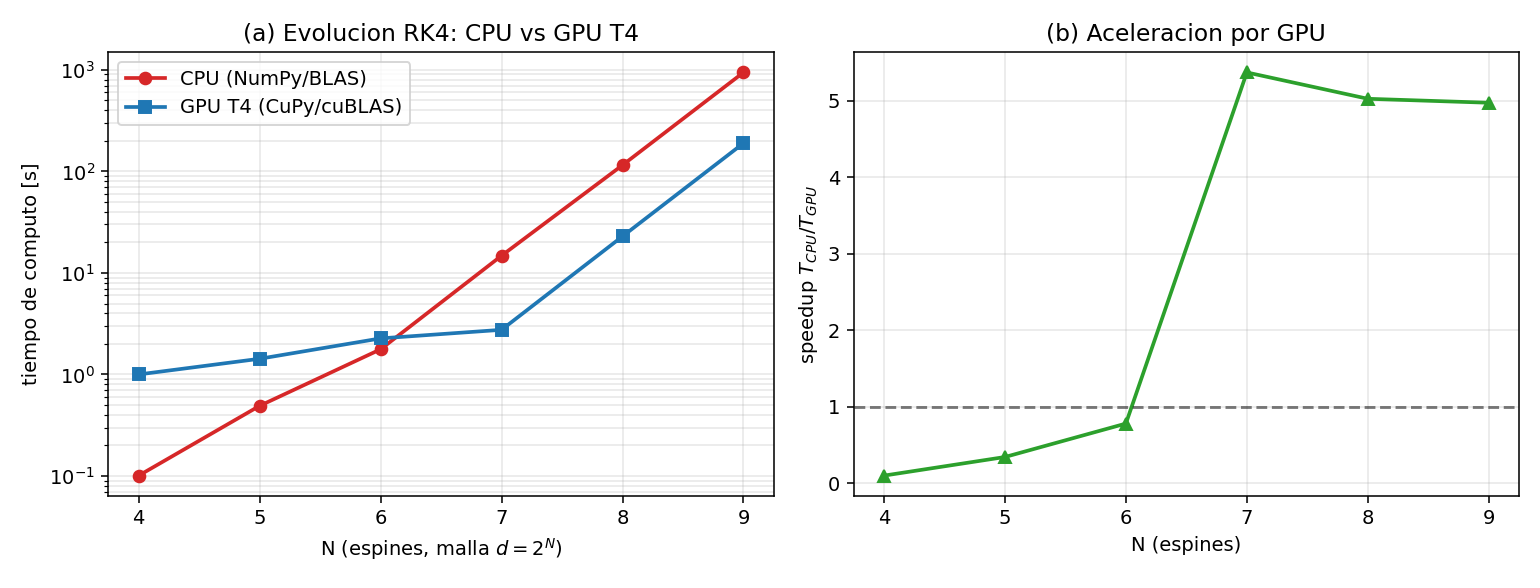
\includegraphics[width=\linewidth]{T2/cuda/results/fig_t2_cuda_evolution.png}\\
    {\scriptsize\textcolor{soft}{Evolución RK4: CPU vs GPU T4 (cuBLAS).}}
  \end{column}
  \begin{column}{0.5\textwidth}\small
    \textbf{Tercer escalón:} serie $\to$ OpenMP $\to$ \cs{CUDA T4}. El \texttt{matmul}
    denso $\to$ cuBLAS \texttt{zgemm}.
    \begin{itemize}\small
      \item GPU pierde a $d$ pequeño (kernels) y \cs{gana $\sim5\times$} a $N\!\ge\!7$
        ($N{=}9$: 943\,s $\to$ 190\,s).
      \item GEMM hasta $250$ GFLOP/s ($d{=}2048$).
      \item Validación triple GPU $=$ CPU $=$ C++ ($D_{HS}\!\to\!0$).
    \end{itemize}
    {\scriptsize\textcolor{soft}{Notebook ejecutado + \texttt{resultados\_t2\_cuda.zip} en \texttt{T2/cuda/}.}}
  \end{column}
  \end{columns}
\end{frame}

% ====================================================================
\divider{juan}{Juan}{6 · Muchos cuerpos: redes tensoriales}

\begin{frame}{T3b — Framework y discretización (TEBD)\J}
  \small
  \textbf{Redes tensoriales} \cite{Weimer2021,Orus2014}. La matriz densidad como un
  \cs{\emph{superket}} $|\rho\rangle\rangle$ --- un MPS de dimensión física 4 por sitio:
  \begin{itemize}
    \item \textbf{TEBD}: se trotteriza $e^{dt\,\Lop}$ en \textbf{compuertas locales} de
      2 sitios y se \textbf{trunca} el enlace a $\chi$ por SVD.
    \item Coste \cs{polinómico en $\chi$} (no exponencial en $N$) $\Rightarrow$ abre
      tamaños imposibles en denso.
    \item \textbf{Paralelización: hilos.} En una capa, los bonds \emph{pares} (o
      impares) son disjuntos; sus SVD ($\mathcal{O}(\chi^3)$) son independientes y numpy
      \cs{libera el GIL}.
  \end{itemize}
\end{frame}

\begin{frame}[fragile]{T3b — Núcleo: serial \textbar\ paralelo (hilos)\J}
  \begin{columns}[T]
  \begin{column}{0.46\textwidth}\centering\textbf{\small Serial}
\begin{lstlisting}[language=Python]
# capa de Trotter
for k in bonds:        # disjuntos
    mps.apply_gate(
        k, gate, chi)  # SVD O(chi^3)
\end{lstlisting}
  \end{column}
  \begin{column}{0.54\textwidth}\centering\textbf{\small Paralelo (ThreadPool)}
\begin{lstlisting}[language=Python]
executor.map(
    lambda k: mps.apply_gate(k, gate, chi),
    bonds)             # SVD libera el GIL
# capas par / impar -> bonds independientes
\end{lstlisting}
  \end{column}
  \end{columns}
  \vfill
  {\small Paralelismo \cs{estructurado}: intermedio entre el SpMV acoplado (T1) y las
  trayectorias independientes (T3). Se mapea a MPI repartiendo segmentos de la cadena.}
\end{frame}

\begin{frame}{T3b — Validación, escalado y alcance\J}
  \begin{columns}[T]
  \begin{column}{0.34\textwidth}\centering
    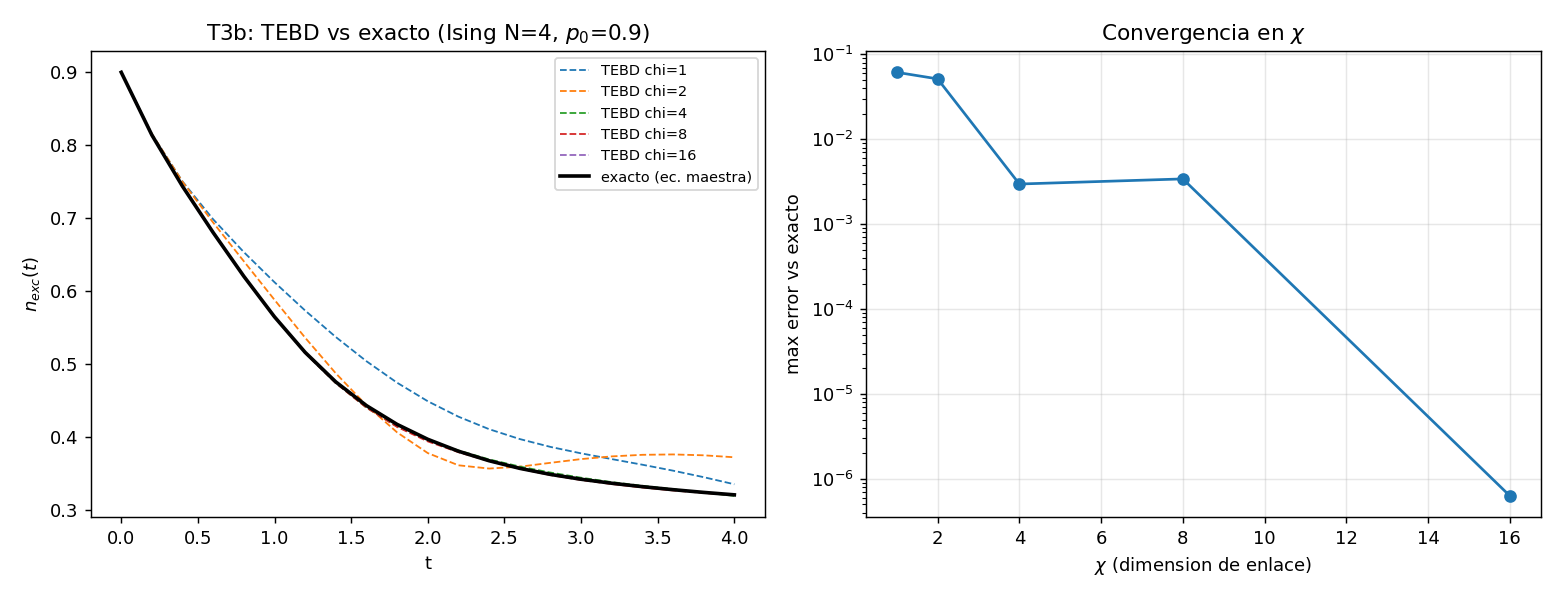
\includegraphics[width=\linewidth]{juan/T3/T3b_tensor_networks/results/t3b_validation.png}\\
    {\scriptsize\textcolor{soft}{Error $\to6\times10^{-7}$ al subir $\chi$.}}
  \end{column}
  \begin{column}{0.34\textwidth}\centering
    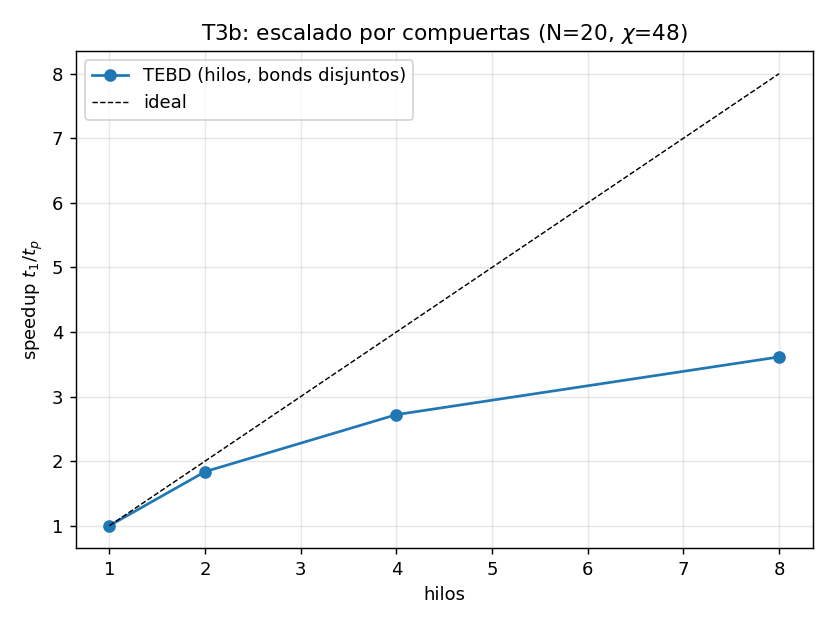
\includegraphics[width=\linewidth]{juan/T3/T3b_tensor_networks/results/t3b_scaling.png}\\
    {\scriptsize\textcolor{soft}{Hilos: $3.6\times$ (8).}}
  \end{column}
  \begin{column}{0.32\textwidth}\small
    \begin{itemize}\small
      \item Validado vs exacto: error controlado por $\chi$.
      \item Escala $\sim3.6\times$ (estructurado).
      \item \cs{$N=32$} ($4^{32}\!\approx\!10^{19}$), imposible en denso, en $\sim$3.6\,s.
    \end{itemize}
  \end{column}
  \end{columns}
\end{frame}

\begin{frame}{T3b — El cruce de Mpemba (redes tensoriales)\J}
  \begin{columns}[T]
  \begin{column}{0.55\textwidth}\centering
    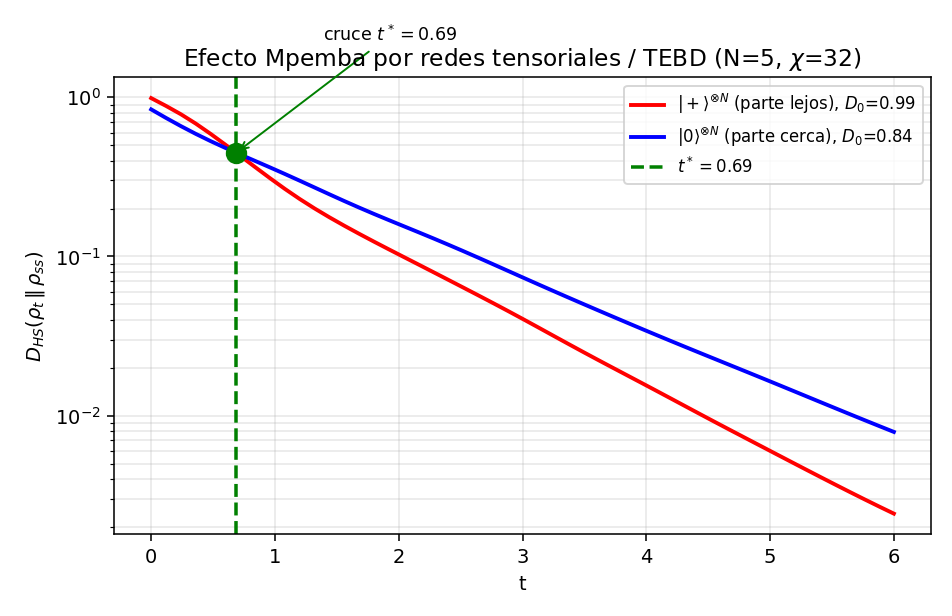
\includegraphics[width=0.92\linewidth]{juan/T3/T3b_tensor_networks/results/fig_t3b_mpemba.png}
  \end{column}
  \begin{column}{0.45\textwidth}\small
    TEBD también reproduce el efecto: $\ket{+}^{\otimes N}$ \textbf{adelanta} a
    $\ket{0}^{\otimes N}$ en \cs{$t^*\approx0.69$}, idéntico a RK4/Krylov (a $\chi$
    grande TEBD es exacto).
    \medskip

    {\scriptsize\textcolor{soft}{Los \textbf{cuatro} métodos de evolución (RK4, Krylov,
    trayectorias, redes tensoriales) dan el mismo $t^*$.}}
  \end{column}
  \end{columns}
\end{frame}

% ====================================================================
\divider{juan}{Juan}{7 · Conclusiones generales}

\begin{frame}{Conclusiones — HPC\J}
  \begin{itemize}
    \item \cj{El patrón de cómputo dicta el paradigma.} Lo vimos como un espectro de
      escalabilidad:
    \begin{itemize}\small
      \item \textbf{T1} SpMV \emph{acoplado} (OpenMP/MPI $\sim2.9\times$, comunicación).
      \item \textbf{T3b} redes tensoriales \emph{estructurado} (hilos $\sim3.6\times$).
      \item \textbf{T3} trayectorias \emph{embarrassingly parallel} (MPI $\sim5.6\times$,
        casi ideal, multinodo).
      \item \textbf{T2} evolución densa $\to$ \cs{GPU} (cuBLAS $\sim5\times$).
    \end{itemize}
    \item Cada paradigma (OpenMP, MPI, hilos, CUDA) elegido por la \emph{estructura del
      algoritmo}, no por moda. \emph{Acoplado $<$ estructurado $<$ independiente.}
  \end{itemize}
\end{frame}

\begin{frame}{Conclusiones — Física\J}
  \begin{itemize}
    \item El efecto Mpemba cuántico es \cs{geometría espectral}: no-normalidad de
      $\Lop$ $+$ criterio $a_2=0$ \cite{Carollo2021}.
    \item \cs{Cruce reproducido por los CUATRO métodos} de evolución (RK4, Krylov,
      trayectorias, redes tensoriales), todos con $t^*\!\approx\!0.69$–$0.75$ ---
      \textbf{validación cruzada} total.
    \item Escalable a muchos cuerpos por dos rutas complementarias (trayectorias y
      redes tensoriales) que llegan a tamaños imposibles en denso.
  \end{itemize}
\end{frame}

% ====================================================================
\divider{seb}{Sebastián}{8 · Relevancia en el efecto macro/meso}

\begin{frame}{Del cuántico al mesoscópico y macroscópico\Sb}
  \begin{columns}[T]
  \begin{column}{0.5\textwidth}\small
    \textbf{La firma es universal.} El mismo mecanismo --- \cs{geometría espectral de
    la relajación} --- explica el cruce en cascadas clásicas, coloides y sistemas
    cuánticos \cite{LuRaz2017,Kumar2022,Teza2026}.
    \medskip

    \textbf{Lo que devuelve el enfoque cuántico:}
    \begin{itemize}\small
      \item Un \emph{criterio operacional} ($a_2=0$) y herramientas HPC para
        \emph{predecir} y \emph{diseñar} el efecto.
      \item Aplicaciones: \cs{termometría cuántica} y enfriamiento acelerado
        \cite{Manikandan2021,Ivander2023}.
    \end{itemize}
  \end{column}
  \begin{column}{0.5\textwidth}\centering
    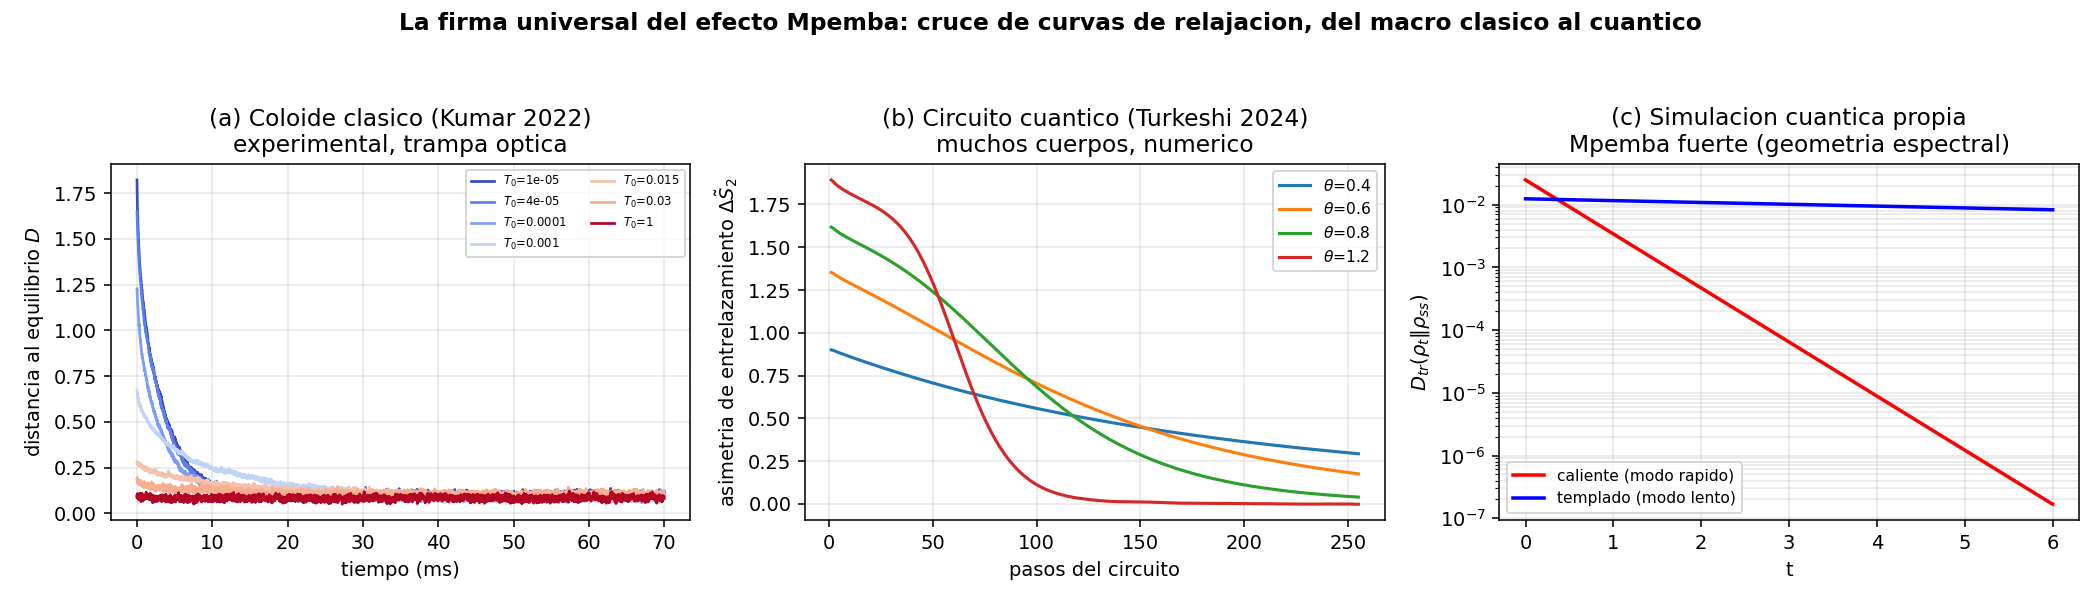
\includegraphics[width=\linewidth]{macro/results/fig_macro_universal.png}\\
    {\scriptsize\textcolor{soft}{La firma universal del cruce: del macro al cuántico.}}
  \end{column}
  \end{columns}
\end{frame}

\begin{frame}[allowframebreaks]{Referencias}
  \scriptsize
  \bibliographystyle{abbrv}
  \bibliography{../context/doc/referencias}
\end{frame}

\begin{frame}[plain]
  \vfill\centering
  {\Large\bfseries ¡Gracias!}\\[6pt]
  {\small \cj{Juan} \;\textbar\; \cs{Sebastián} \quad ---\quad Efecto Mpemba cuántico en HPC}
  \vfill
\end{frame}

\end{document}
